\documentclass{beamer}
\usetheme{Boadilla}
\usecolortheme{beaver}
\usepackage[english]{babel}
\usepackage{csquotes}
\usepackage[backend=biber,style=numeric-comp,sorting=none]{biblatex}
\usepackage{amsmath}
\usepackage{graphicx}
\usepackage{float}
\usepackage{multirow} % needed for tables
\usepackage{xcolor}
\usepackage{caption}
\usepackage{subcaption}
\usepackage{algorithm}
\usepackage{algpseudocode}
\usepackage{float}
\usepackage{amsthm}
\usepackage{algorithm}
\usepackage{algpseudocode}
\usepackage{amssymb}
\bibliography{bibliography}

\graphicspath{{../pdf/}{../MMPics/}}
\addbibresource{../references.bib}

\newcommand\at[2]{\left.#1\right|_{#2}}

\AtBeginSection[]{
  \begin{frame}
  \vfill
  \centering
  \begin{beamercolorbox}[sep=8pt,center,shadow=true,rounded=true]{title}
    \usebeamerfont{title}\insertsectionhead\par%
  \end{beamercolorbox}
  \vfill
  \end{frame}
}

\title{Martingale Matching}
\subtitle{A novel approach to diffusion}
\author{Anton von Nandelstadh}
\institute{Uppsala University}
\date{\today}

\begin{document}

\begin{frame}
\titlepage
\end{frame}

\begin{frame}{Outline}
	\tableofcontents
\end{frame}

\section{SDE Background}
\begin{frame}
\begin{definition}[Filtration]
	Let $(\Omega, \mathcal{F}, P)$ be a probability space and let $T$ be an index set. For each $i \in T$, let $\mathcal{F}_i$ be a sub-$\sigma$-algebra of $\mathcal{F}$. Then $\{\mathcal{F}_i\}_{i \in T}$ is a filtration if $\mathcal{F}_k \subset \mathcal{F}_l$ for each $k \leq l$. Then $(\Omega, \mathcal{F}, \{\mathcal{F}_t\}, P)$ is called a filtered probability space.
\end{definition}
\end{frame}

\begin{frame}
\begin{definition}[Martingale]
	A stochastic process $X:T \times \Omega \to \mathbb{R}$ on probability space $(\Omega, \mathcal{F}, P)$ is a martingale w.r.t. the filtration $\{\mathcal{F}\}$ (of $(\Omega, \mathcal{F}, P)$) if
	\begin{enumerate}
		\item
		X is adapted to the filtration. That is, $X_t$ is $\mathcal{F}_t$ measurable for each $t \in T$.
		\item
			for each $t$, $\mathbb{E}[X_t] < \infty$
		\item
			for all $s$ and $t$ with $s < t$, $\mathbb{E}[X_t|\mathcal{F}_s] = X_s.$
	\end{enumerate}
\end{definition}
\end{frame}

\begin{frame}
	\begin{definition}[Brownian motion]
		Brownian motion is a stochastic process $\{B_t\}$ such that
		\begin{itemize}
			\item $B_0 = 0$
			\item for all $k$, and all $0 < t_1 < \ldots < t_k$, the random variables \[B_{t_k} - B_{t_{k-1}} \sim N(0, t_k - t_{k-1})\] are independent
			\item $B_t$ is almost surely continuous in $t$
		\end{itemize}
	\end{definition}
\end{frame}

\begin{frame}
\begin{definition}[Itô integral]
	Let $f \in \nu(S,T)$. Then the Itô integral of $f$ (from $S$ to $T$) is defined by
	\begin{equation}
		\int_S^T f(t, \omega)dB_t(\omega) = \lim_{n \to \infty} \int_S^T \phi_n(t_, \omega)dB_t(\omega)
	\end{equation}
	where $\{\phi_n\}$ is a sequence of elementary functions such that
	\begin{equation}
		\mathbb{E}\left[\int_S^T(f(t, \omega) - \phi_n(t, \omega))^2dt\right] \to 0 \quad \text{as } n \to \infty
	\end{equation}
\end{definition}
\end{frame}

\begin{frame}
\begin{definition}[Stochastic differential equation]
	A process $X_t$ satisfies the stochastic differential equation
	\begin{equation}
		dX_t = b(t, X_t)dt + \sigma(t, X_t)dB_t
	\end{equation}
	if it satisfies the integral equation
	\begin{equation}
		\label{eq:sde}
		X_t = X_0 + \int_0^t b(s, X_s) ds + \int_0^t \sigma (s, X_s) dB_s
	\end{equation}
\end{definition}
\end{frame}

\begin{frame}
\begin{theorem}[Existence and uniquencess of SDEs (Part 1)]
	\label{thm:existence}
	Let $T>0$ and $b:[0,T] \times \mathbb{R}^n \to \mathbb{R}^n, \sigma:[0, T] \times \mathbb{R}^n \to \mathbb{R}^{n \times m}$ be measurable functions satisfying
	\begin{equation}
		|b(t, x)| + |\sigma(t, x)| \leq C(1 + |x|) \quad x\in\mathbb{R}^n, t\in [0,T]
	\end{equation}
	for some constant $C$, $|\sigma|^2 = \sum|\sigma_{ij}|^2$, and such that
	\begin{equation}
		|b(t, x) - b(t,y)| + |\sigma(t,x)-\sigma(t,y)| \leq D|x-y| \quad x,y\in \mathbb{R}^n, t\in[0,T]
	\end{equation}
	for some constant D. Let Z be a random variable which is independent of the $\sigma$-algebra $F_\infty$ generated by $B_s$, $s \geq 0$, and such that
	\begin{equation}
		\mathbb{E}[|Z|^2] < \infty.
	\end{equation}
\end{theorem}
\end{frame}

\begin{frame}
\begin{theorem}[Existence and uniquencess of SDEs (Part 2)]
	Then the stochastic differential equation 
	\begin{equation}
		dX_t = b(t, X_t)dt + \sigma(t, X_t)dB_t, \quad 0 \leq t \leq T, X_0 = Z
	\end{equation}
	has unique continuous (in t) solution $X_t$ with the property that $X_t$ is adapted to the filtration $\mathcal{F}_t^Z$ generated by $Z$ and $B_s, s \leq t$ and
	\begin{equation}
		\mathbb{E}\left[ \int_0^T |X_t|^2 dt\right] < \infty.
	\end{equation}
\end{theorem}
\end{frame}

\begin{frame}
\begin{definition}[Time-homogenous Itô diffusion]
	A (time-homogenous) Itô diffusion is a stochastic process $X_t(\omega) = X(t,\omega):[0,\infty) \times \Omega \to \mathbb{R}^n$ satisfying a stochastic differential equation of the form
	\begin{equation*}
		dX_t = b(X_t)dt + \sigma(X_t)dB_t, \quad t \geq s; X_s = x
	\end{equation*}
where $B_t$ is m-dimensionsal Brownian motion and $b:\mathbb{R}^n \to \mathbb{R}^n$, $\sigma:\mathbb{R}^n \to \mathbb{R}^{n \times m}$ satisfy

\begin{equation*}
	|b(x) - b(y)| + |\sigma(x) - \sigma(y)| \leq D|x-y|; \quad x,y \in \mathbb{R}^n
\end{equation*}

We call $b$ the drift coefficient and $\sigma$ the diffusion coefficient.
\end{definition}
\end{frame}

\begin{frame}
\begin{theorem}[Itô's lemma]
	Let
	\begin{equation*}
		dX(t) = u dt + v B(t)
	\end{equation*}
	be an n-dimensional Itô process. Let $f(t, x)$ be a $C^2$ map from $[0,\infty) \times \mathbb{R}^n$ into $\mathbb{R}$. Then the process

	\begin{equation*}
		Y(t, \omega) = f(t, X(t))
	\end{equation*}

	is again an Itô process, given by

	\begin{equation*}
		dY = \frac{\partial f}{t}(t,X)dt = \sum_{i}\frac{\partial f}{\partial x_i}(t, X)dX_i + \frac{1}{2}\sum_{i,j}\frac{\partial^2f}{\partial x_i \partial x_j} dX_i dX_j
	\end{equation*}

	where $dB_i dB_j = \delta_{i,j}dt$, $dB_idt = dtdB_i = dtdt = 0$.
	
\end{theorem}
\end{frame}

\begin{frame}
\begin{definition}[Generator]
	Let $\{X_t\}$ be an Itô diffusion in $\mathbb{R}^n$. The generator $\mathcal{L}$ of $X_t$ is defined by
	\begin{equation*}
		\mathcal{L}f(x) = \lim_{t \downarrow 0}\frac{\mathbb{E}^x[f(X_t)] - f(x)}{t}; \quad x \in \mathbb{R}^n
	\end{equation*}
	for the set of functions $f:\mathbb{R}^n \to \mathbb{R}$ where the limit exists uniformly.
\end{definition}
\end{frame}

\begin{frame}
	\begin{theorem}[Diffusion generator]
	\label{thm:diffgen}
The generator of the diffusion process is given by

\begin{equation*}
	\mathcal{L}_s f = b \cdot \nabla f + \frac{1}{2} \mathrm{tr}(\sigma\sigma^T \nabla^2 f)	
\end{equation*}

which in the case where $\sigma$ is a constant simplifies to 

\begin{equation*}
	\mathcal{L}_s f = b \cdot \nabla f + \frac{1}{2} \sigma^2 \Delta f	
\end{equation*}

Here $f$ is any $C^2$ function.
\end{theorem}
\end{frame}

\begin{frame}
	\begin{block}{Proof}
	The Itô formula gives
	\begin{equation*}
		df(X_t) = \sum_i b_i \frac{\partial f}{\partial x_i} + \frac{1}{2}\sum_{i,j}(\sigma \sigma^{T})_{i,j} \frac{\partial f}{\partial x_i \partial x_j}dt + M_t
	\end{equation*}

	where $M_t$ is some martingale term. We rewrite this as 

	\begin{equation*}
		f(X_t) = f(x) + \int_0^t \mathcal{L}f(X_s)ds + M_t
	\end{equation*}

	and we now wish to show that $\mathcal{L}f$ is the generator.
	\end{block}
\end{frame}

\begin{frame}
	\begin{block}{Proof contd.}
	Taking expectations we have

	\begin{equation*}
		T_tf(x) = f(x) + \int_0^t \mathbb{E}_x[\mathcal{L}f(X_s)]ds + \mathbb{E}[M_t]
	\end{equation*}

	so that 

	\begin{equation*}
		T_tf(x) - f(x) = \int_0^t T_s (\mathcal{L}f)(x)ds
	\end{equation*}

	which gives us that

	\begin{equation*}
		\at{T_t\frac{d}{dt}f(x)}{t=0} = \mathcal{L}f(x)
	\end{equation*}

	and so it is clear that $\|\frac{d}{dt}T_tf - \mathcal{L}f\|$ as $t \to 0$.
	\qed
\end{block}
\end{frame}

\section{Generative Models and Diffusion}

\begin{frame}
\begin{definition}[Generative modelling]
	Generative modelling is the process of training a model to transform a sample from a simple distribution $p_{simple}$ to a data distribution $p_{data}$. 
\end{definition}
\begin{definition}[Dataset]
	A dataset is a finite number of samples $z_1,\ldots,z_N \sim p_{data}$.
\end{definition}
\begin{definition}[Probability path]
	A probability path is a time-dependent probability $\{p_t\}_{0 \leq t \leq 1}$.
\end{definition}
\end{frame}

\begin{frame}
\begin{definition}[Diffusion model]
	A diffusion model is given by:
	\begin{align*}
		dX_t &= b_t^{\theta}(X_t)dt + \sigma_t d W_t \\
		X_0 &\sim p_{simple}
	\end{align*}
	where $b_t^{\theta}:\mathbb{R}^d \to \mathbb{R}^d$ is the parametrized drift, $\sigma_t: \mathbb{R}^d \to \mathbb{R}$ is our diffusion coefficient at time t, and $p_{simple}$ is our initial data distribution.
\end{definition}
\begin{block}{Aim}
	The goal is to find coefficients $b_t^{\theta}$ and $\sigma_t$ such that $X_1 \sim p_{data}$.
\end{block}
\end{frame}

\section{Algorithm}

\begin{frame}
\begin{theorem}
$M_t^f$ is a martingale where

\begin{equation}
	\label{eq:mart}
	M_t^f = f(X_t) - f(X_0) - \int_0^t \mathcal{L}_s f(X_s) ds 
\end{equation}

so that $\mathbb{E}[M_t^f] = 0$. Here $f \in C^2$ is an arbitrary test function. $\mathcal{L}_s$ is the generator of the diffusion process.
\label{thm:mart}
\end{theorem}

\begin{proof}
	This follows from the proof of the diffusion generator.
\end{proof}
\end{frame}

\begin{frame}
	\begin{block}{Naive residual}
\begin{equation*}
	\tilde R_{t_k}^{f,i} = f(X_{t_{k+1}}^i) - f(X_{t_k}^i) - \int_{t_k}^{t_{k+1}}\mathcal{L}_sf(X_s^i)ds
\end{equation*}
\end{block}

\begin{block}{Naive loss function}
\begin{equation}
	\label{naive_loss}
	L_1 = \frac{1}{T|\mathcal{F}|} \sum_{k=1}^{T} \sum_{f \in \mathcal{F}} \left(\frac{1}{N}\sum_{i=1}^{N} \tilde R^{f, i}\right)^2
\end{equation}
\end{block}
\end{frame}

\begin{frame}
\begin{block}{Monte-Carlo loss function}
\begin{equation}
	\label{bad_loss}
	L_2 = \frac{1}{|\mathcal{F}|} \sum_{f \in \mathcal{F}} \left(\frac{1}{N}\sum_{i=1}^{N} \tilde R^{f, i}\right)^2
\end{equation}
\end{block}
\end{frame}

\begin{frame}
\begin{block}{Weak residual}
\begin{equation}
	R_{t_k}^{f,i} = f(Y_{t_{k+1}}^i) - f(X_{t_k}^i) - \int_{t_k}^{t_{k+1}}\mathcal{L}_sf(X_s^i)ds
\end{equation}

where $Y_{t_{k+1}} \sim p_{t_{k+1}}(\cdot|z)$ and $X_{t_k} \sim p_{t_k}(\cdot|z)$.
\end{block}

\begin{block}{Weak loss}
\begin{equation}
	\label{better_loss}
	\tilde L_3 = \frac{1}{|\mathcal{F}|} \sum_{f \in \mathcal{F}} \left(\frac{1}{N}\sum_{i=1}^{N} R^{f, i}\right)^2
\end{equation}
\end{block}

\begin{theorem}
	Minimizing equation \ref{better_loss} implies weak generator learning. Explicitly, if for each $f \in \mathcal{F}$ we have that $\mathbb{E}[R^f_t] = 0$, then \[\mathbb{E}[\mathcal{L} f(X_t)] = \mathbb{E}[\mathcal{L}^\theta f(X_t)]\] for each $f \in \mathcal{F}$.
\end{theorem}
\end{frame}

\begin{frame}

\begin{proof}
	Using Thm. \ref{thm:mart}, we find that
	\begin{align*}
		\mathbb{E}[R_t] &= \mathbb{E}[f(Y_{t+\Delta t})] - \mathbb{E}[f(X_t)] - \int_t^{t+\Delta t} \mathbb{E}[\mathcal{L}^\theta f(X_s)]ds \\
						&= \mathbb{E}[f(Y_0)] + \int_0^{t+\Delta t} \mathbb{E} [\mathcal{L}f(Y_s)] ds - \mathbb{E}[f(X_0)] - \int_0^{t} \mathbb{E}  [\mathcal{L}f(X_s)] ds \\ &- \int_t^{t+\Delta t} \mathbb{E}[\mathcal{L}^\theta f(X_s)]ds \\
							 &= \int_t^{t+\Delta t} \mathbb{E}[\mathcal{L} f(X_s) - \mathcal{L}^\theta f(X_s)]ds \\
							 &\approx \Delta t \mathbb{E}[\mathcal{L} f(X_t) - \mathcal{L}^\theta f(X_t)]
	\end{align*}
	Here we use Fubini's theorem, since the generator is integrable, and we use that $X_s$ and $Y_s$ follow the same distribution to get cancellations.
\end{proof}
\end{frame}

\begin{frame}
	\begin{block}{Error estimation}
	If we now write $\epsilon = \mathbb{E}[\mathcal{L}f(X_t) - \mathcal{L}^\theta f(X_t)]$ as our error, then 

	\begin{equation}
		\min_\theta \left( \frac{1}{N} \sum_{i=1}^n R_\theta^{f, i}\right)^2 \sim {\Delta t}^2 \epsilon^2
		\label{eq:order}
	\end{equation}
	\end{block}
\end{frame}

\begin{frame}
	\begin{block}{Decomposition}
\[
    \mathbb{E}\bigl[(R_\theta^f)^2\bigr]
    =
    \bigl(\mathbb{E}[R_\theta^f]\bigr)^2
    +
    \operatorname{Var}(R_\theta^f),
\]
	\end{block}

	\begin{block}{Martingale error}
		\begin{equation}
			\label{best_loss}
			L_{ME} = \frac{1}{|\mathcal{F}|N} \sum_{f \in \mathcal{F}} \sum_{i=1}^{N} (R^{f, i})^2.
		\end{equation}
	\end{block}
\end{frame}

\begin{frame}
	\begin{algorithm}[H]
	\caption{Martingale Matching}\label{alg:mm}
	\begin{algorithmic}
		\Require Neural net $b_t^{\theta}$, diffusion coefficient $\sigma$, time-step $\Delta t$, dataset of samples $z \sim p_{data}$, conditional probability path $p_t(\cdot|z)$
		\For{each mini-batch of data}
		\State Sample datum z from dataset.
		\State Sample $t \sim U[0,1-\Delta t]$.
		\State Set $x_t \sim p_t(.|z)$, $x_{t+\Delta t} \sim p_{t + \Delta t}(.|z)$
		\State Compute loss $\mathcal{L}_{ME}^\theta$
		\State Update the model parameter $\theta$ via gradient descent on $\mathcal{L}_{ME}^{\theta}$
		\EndFor	
	\end{algorithmic}
\end{algorithm}
\end{frame}

\begin{frame}
\begin{definition}[Random Fourier features]
	A random Fourier feature is a function of the type 
	\begin{equation*}
		f_{\omega_1}(x) = cos(w^\intercal x) \quad f_{\omega_2}(x) = sin(w^\intercal x)
	\end{equation*}
	where $x \in \mathbb{R}^d$ and $\omega \sim N(0, \sigma^2 I_d)$.
\end{definition}
\end{frame}

\begin{frame}
\begin{definition}[Polynomial test functions]
	Suppose our dataset has dimension $n$, and we want to consider polynomials of degree $d$. The the set of polynomial test functions is
	\begin{equation*}
	\{f(x) = x^k_ix^k_j | i,j \in \{0,\ldots,n\}, k \in \{0,\ldots, d\}\}.
\end{equation*}
\end{definition}
\end{frame}

\begin{frame}
\begin{definition}[Gaussian probability path]
	Let $\alpha_t = \alpha(t) \in C^1([0,1])$ and $\beta_t = \beta(t) \in C^1([0,1])$ be noise schedulers, that is, monotonic functions with $\alpha_0 = \beta_1 = 0$ and $\alpha_1 = \beta_0 = 1$. We then define the Gaussian conditional probability path to be

	\begin{equation*}
		p_t(\cdot|z) = N(\alpha_tz, \beta_t^2 I_d).
	\end{equation*}

	Then this probability path fulfills the boundary conditions
	\begin{equation*}
		p_0(\cdot|z) = N(\alpha_0z, \beta_0^2 I_d) = N(0, I_d)\quad and \quad p_1(\cdot|z) = N(\alpha_1 z| \beta_1^2 I_d) = N(z,0) 
	\end{equation*}
\end{definition}
\end{frame}

\begin{frame}
\begin{algorithm}[H]
	\caption{Euler-Maruyama}\label{alg:euler}
	\begin{algorithmic}
		\Require Neural net $b_t^{\theta}$, number of steps n, diffusion coefficient $\sigma_t$
		\State Set $h = \frac{1}{n}$
		\State Set $t=0$
		\State Sample $X_0 \sim p_{simple}$
		\For{$i = 1, \ldots, n$}
		\State Sample $\epsilon \sim N(0, I)$
			\State $X_{t+h} = X_t + h b_t^{\theta} (X_t) + \sigma_t \sqrt{h} \epsilon$
			\State Update $t \leftarrow t + h$
		\EndFor
		\State \Return $X_1$
	\end{algorithmic}
\end{algorithm}
\end{frame}



\section{Results}
\begin{frame}
\begin{figure}[H]
  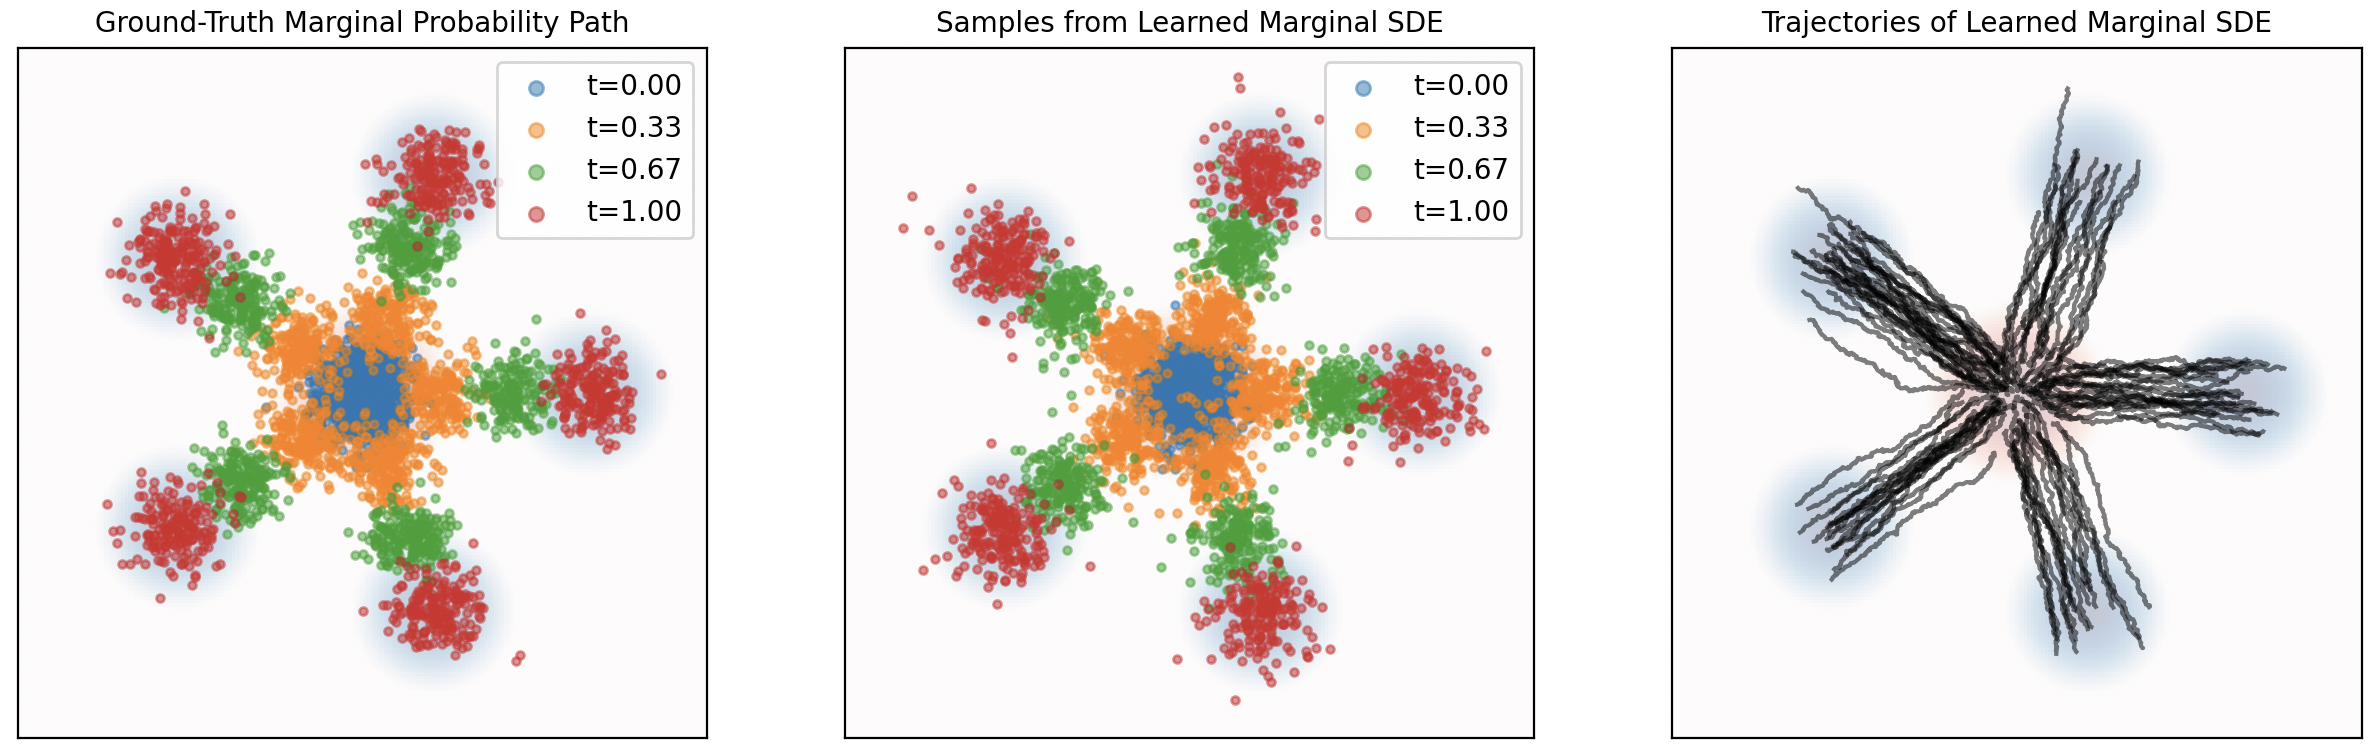
\includegraphics[width=\linewidth]{gauss.png}
  \caption{Learning multiple Gaussians}
  \label{fig:gaussF}
\end{figure}
\end{frame}

\begin{frame}
\begin{figure}[H]
  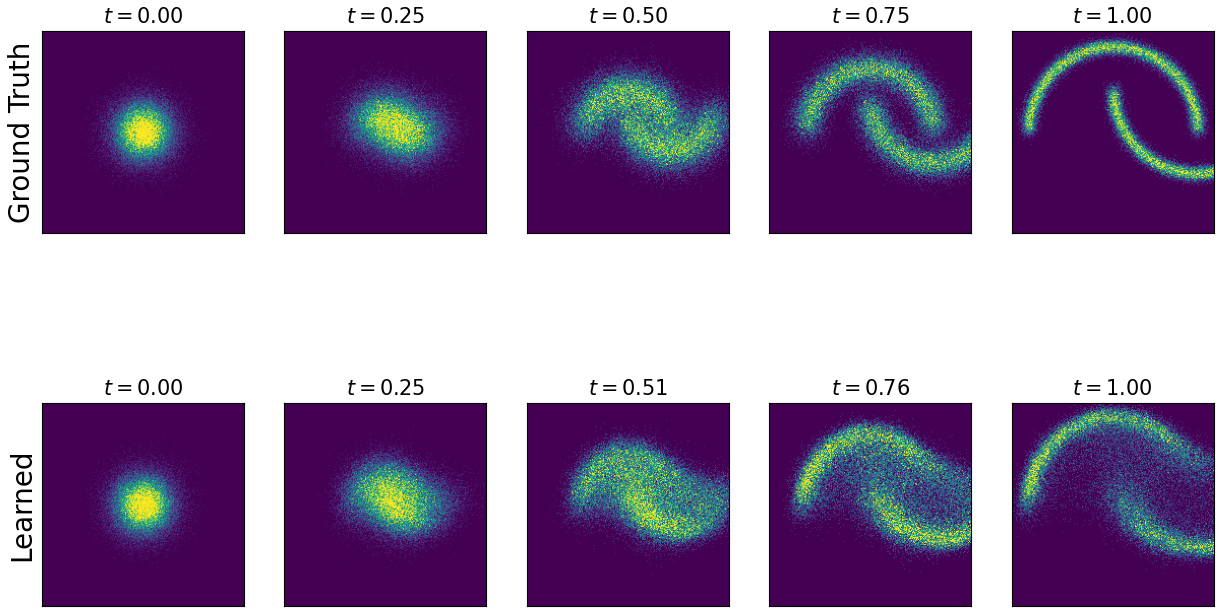
\includegraphics[width=\linewidth]{moons_fourier.png}
  \caption{Learning two moons with Fourier test functions}
  \label{fig:moonF}
\end{figure}
\end{frame}

\begin{frame}
\begin{figure}[H]
  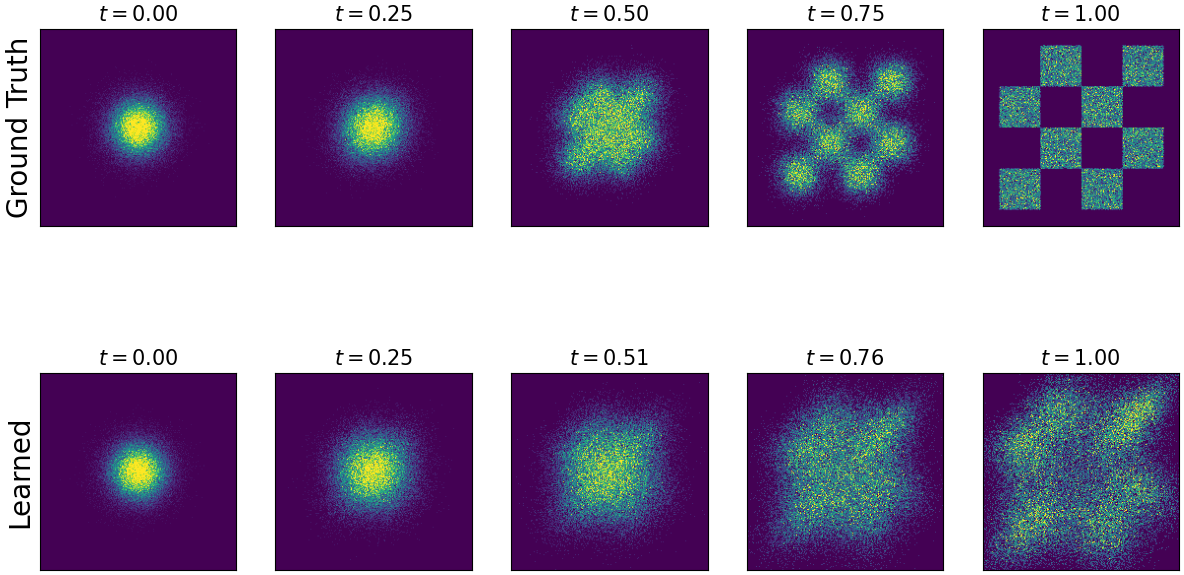
\includegraphics[width=\linewidth]{checkerboard_fourier.png}
  \caption{Learning a checkerboard with Fourier test functions}
  \label{fig:checkF}
\end{figure}
\end{frame}

\begin{frame}
\begin{figure}[H]
  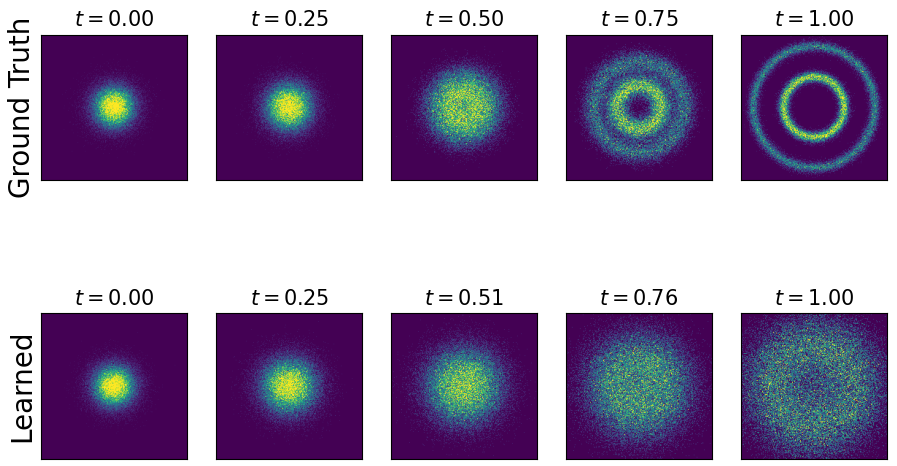
\includegraphics[width=\linewidth]{circles_fourier.png}
  \caption{Learning circles with Fourier test functions}
  \label{fig:circlesF}
\end{figure}
\end{frame}

\begin{frame}
\begin{figure}[H]
  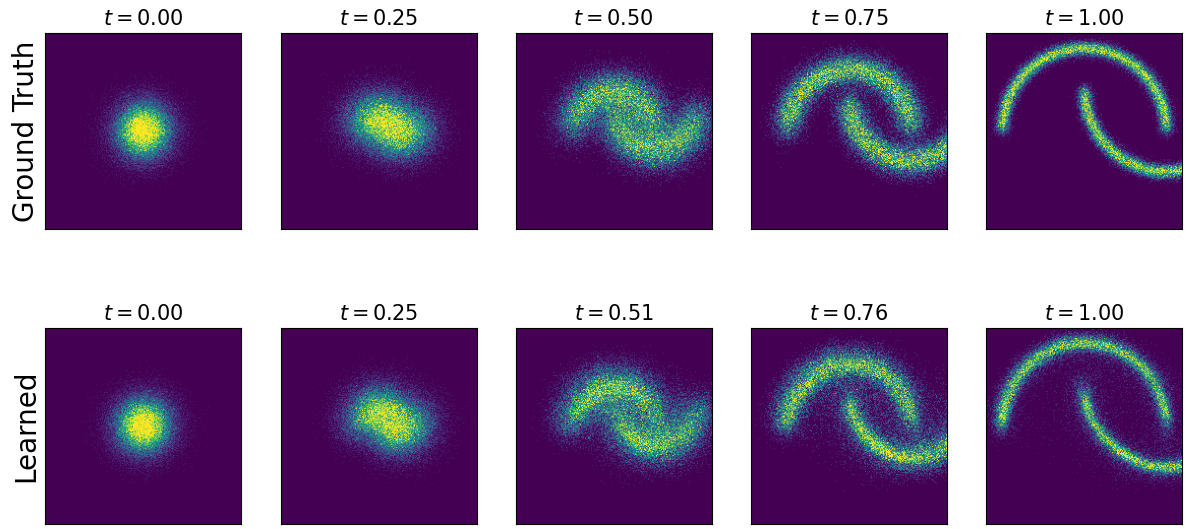
\includegraphics[width=\linewidth]{moons_poly.png}
  \caption{Learning two moons with polynomial test functions}
  \label{fig:moonP}
\end{figure}
\end{frame}

\begin{frame}
\begin{figure}[H]
  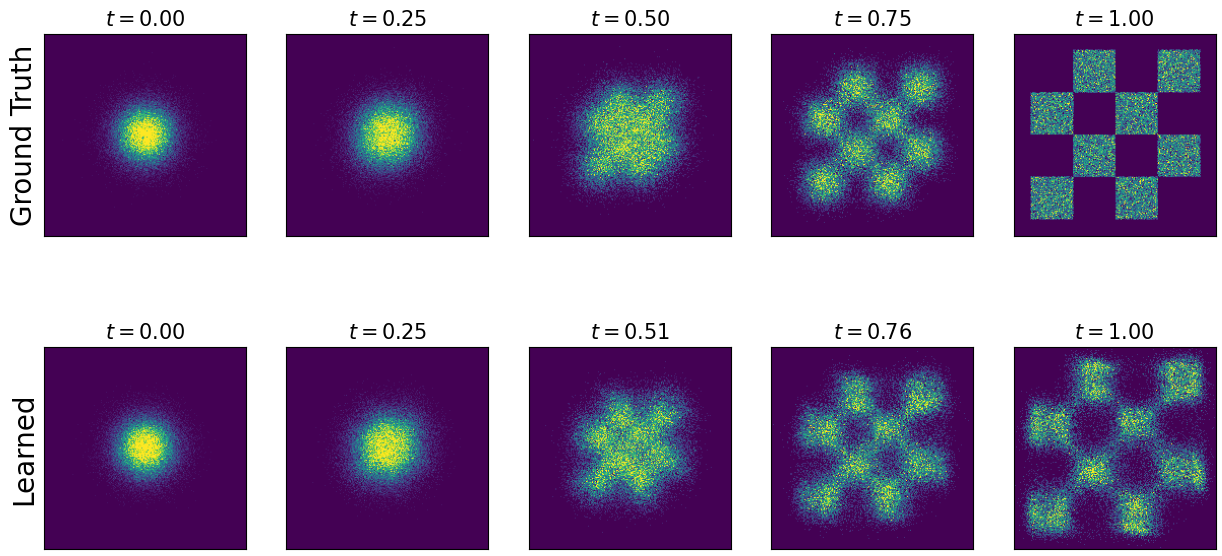
\includegraphics[width=\linewidth]{checkerboard_poly.png}
  \caption{Learning a checkerboard with polynomial test functions}
  \label{fig:checkP}
\end{figure}
\end{frame}

\begin{frame}
\begin{figure}[H]
  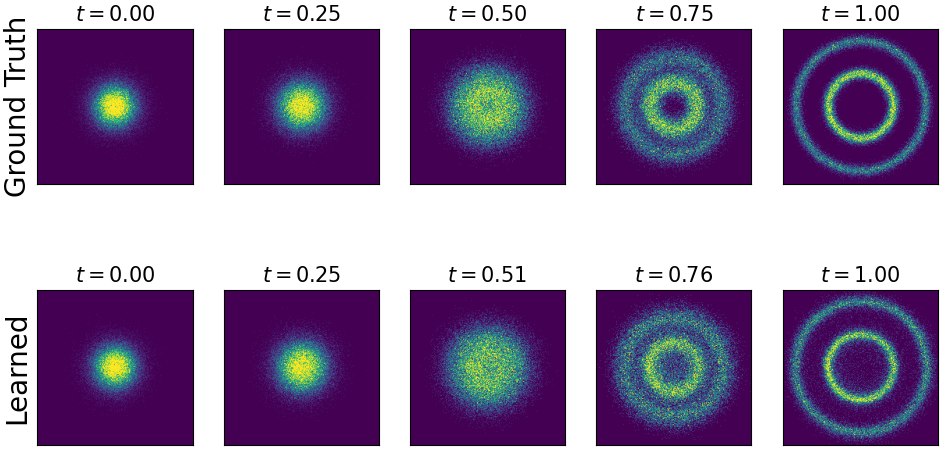
\includegraphics[width=\linewidth]{circles_poly.png}
  \caption{Learning circles with polynomial test functions}
  \label{fig:circlesP}
\end{figure}
\end{frame}

\begin{frame}
	\begin{block}{Conclusion}
		\begin{itemize}
			\item We get excellent results for lower dimensional data
			\item Polynomial test functions expensive in higher dimensions
		\end{itemize}
	\end{block}
	\begin{block}{Extensions}
		\begin{itemize}
			\item Combining test functions
			\item Learning the test functions
			\item More thorough analysis of what test functions learn what
		\end{itemize}
	\end{block}
\end{frame}

\begin{frame}[allowframebreaks]
	\frametitle{References}
	\nocite{*}
	\printbibliography

\end{frame}
\end{document}
